\documentclass[../main.tex]{subfiles}

\begin{document}
\chapter{Goals and thesis scope}

Following document investigates position finding system implementation basing on consumer grade smartphone and network of reference points using Bluetooth Low Energy technology.

As part of the work, there are presented currenty known position finding solutions within underground environment, available technologies and a method of position finding for consumer grade smartphones in underground installations is proposed. There are presented test cases and experiments supported by data analysis from measurements of given factors of the solution. Experiments are focused on stability, repeatability, accuracy and reliability factors. The work do not discuss the mining model representation but general architecture and data exchange model. but there are proposed soluin terms of the location of the reference points, the location of the miner (system user), the safety points and the evacuation exits. The model should allow both the user to navigate to the nearest safety point, taking into account the current state of the corridors, and to allow presentation of the current position in graphical form. As part of the work, a complete model of the solution are be proposed along with the prototype of application for the mobile device. Finally, there are proposed future works that would base on a concept of integration of the location system with the function of remotely updating corridors. There are be provided example use cases.

\chapter{Underground envioronment description}

Underground installations are specific environment in terms of electromagnetic waves propagation, their diamensions, varying accross the tunnels, large scale, weak light, available communication technologies, environmental parameters like humadity, temperature, substances that make up the atmosphere and safety restrictions that limits electronic equipment that can be used on site.

As for the position finding problem in indoor environments there were already developed sucessful solutions, the underground environment make some of assumptions no more valid. That is because of the propagation channel which is difficult to model due to the fact that signals are absorbed by earthen walls, bounce off uneven surfaces, and must pass equipment and other obstacles in corridors.

Description of:
\begin{itemize}
	\item Construction (very briefly):
	\begin{itemize}
		\item how can look like: from complicated (room and phillar) to simple (tunneling)
		\item distances
		\item how big it is: corridor diamensions, room diamanesions, etc.
	\end{itemize}
	\item Conditions in therms of light and air.
	\item What wireless communication methods are available?
\end{itemize}

Answer questions:
\begin{itemize}
	\item if we need the navigation in whole installation? if yes, why?
	\item if we need the navigation only in some places inside installation? if yes, why?
	\item what factors may require from navigation system its extensive lifetime?
\end{itemize}

\section{Underground installation characteristics}

This section covers a short description of underground installations in general that are the environment for the positioning system.

Underground installation therm is a general description of places such as tunnels and shafts that were digged into the earth in purpose of valuable material extraction, transportation, touristics or other reasons. The common phase in those installations is the phase of their creation. There is a need to digg tunnel or shaft at first in order to reach buried ore deposits or just remove not needed rock. Tunnels and shafts are used in this phase to supply material needed to perform exchavation, for personel transportation and rock transportation to the surface. Mining installations are about continous rock exchavation process (creation phase) while the others, like designed for transporation, ends creation phase and moves to the phase of use and maintenance. Underground installations that can be descibed as a gorup of laneways (main and branch tunnels) and in case of mine: mining areas and mined-out areas.

What is the common in underground installation is that there are no reference objects like plants, horizon or sun. Corridors and chambers are almost identical, in particular if there is room-and-pillar extraction method used. For orientation special numbering is introduced in order to identify corridor and given meter of the corridor. Symbols are painted on the walls with reflective paint and are regurally repainted. Dust combined from moisture deposit himself on a substrate, the walls and ceiling covering symbols describing the hallways. It worsens the orientation.

As the purpose of underground installation may be different, there are also different environmental characteristics such as diamensions, type of material (rock), amount of dust, how freqent is in use, what means of communication are placed into, what machines (if any) are being used inside. Along greater depths, the work conditions are decreasing. The probability of coal and gas outbursts increases because of bigger gas emission on deeper levels. Underground installations can be affected also by water leaks, coal dust explosions and rock bursts \cite{WSN_monitoring}. That is why underground installations are prepared for such disasters as floods, fire, high/low pressure, presence of gas, big carbon monoxide (CO) level, or enormous amount of dust. The another risk is connected to people and material transportation. Poor light and narrow working space causes underground car accidents.

Underground mines, which are characterized by their tough working conditions and hazardous environments, require reliable underground installation-wide communication systems in order to prevent from accident if possible or provide means of early warning of possible disaster \cite{Book_wireless_in_mines}. Besides safety purpose, both analog and digital communication is used in order to ensure smooth functioning of workings. For example it is possible to save the machine breakdown time thanks to immediate messages passing  from the vicinity of underground working area to the surface for day-to-day normal operations.

With respect of the areas of the underground working activity there are different communication system used. Communication technology in underground installations use wired transmission media (twisted pair, coaxial, trolley, leaky feeders, and fiber optic cables), wireless and through-the-earth (very low frequency radio methods) transmissions. In most cases the communication solutions are based on wired technologies. Wireless communication techonologies are used in places that are inaccessible or in places affected by disaster where wired communication got broken. It is also havily used for communication purposes with modern underground equipment such as self-propelled mining machines. Wireless communication is installed also in underground installations where probability of disaser is low as an extension to wired technology. Commercial tunneling equip thier corridors with wireless communication technologies such as GSM and WiFi in order to speed up communication between executives on tunel construction site and on surface. Tunneling is about digggin a corridors for transportation purposes in difficoult terrains such as mountains or bellow the water. Operations that are performed it high latitudes where gas is not present are safer then in mines which operates deep under the surface.

There is no standard position marking convetion that are used accross the underground installations. Details about shape, size and current deep and length of corridors are often trated as a company secret as well as their labels. Generally speaking underground installactions are labeled with use of sector name, corridor name and a number of meters since beggining of the corridor. Position within given corridor can be labeled with use of corridor name and the meter, for example $C1-25$, where $C1$ denotes corridor name and $25$ denotes number of meters. Corridor/meter pairs for denoting the position are suffincient in case of not complicated structure of corridors and shafts as well as in complex structured like in case of \textit{room and pillar} layout. Example of room and pillar corridors layout is presented on the figure \ref{fig:room_and_pillar_scheme}. $A1$ denotes transportation corridor. It can be used for example by drill rigs or load-haul-dump machines that are doing the excavation. $S1, S2, S3, ...$ are corridor names within the production block. Entrance to the production block can be named with use of cardinal directions like south in case of the figure \ref{fig:room_and_pillar_scheme}. Pillar diamensions may vary with respect of depth that works are being performed and the type of rock. Pillars can be 20 m -- 40 m thick.

\begin{figure}[ht]
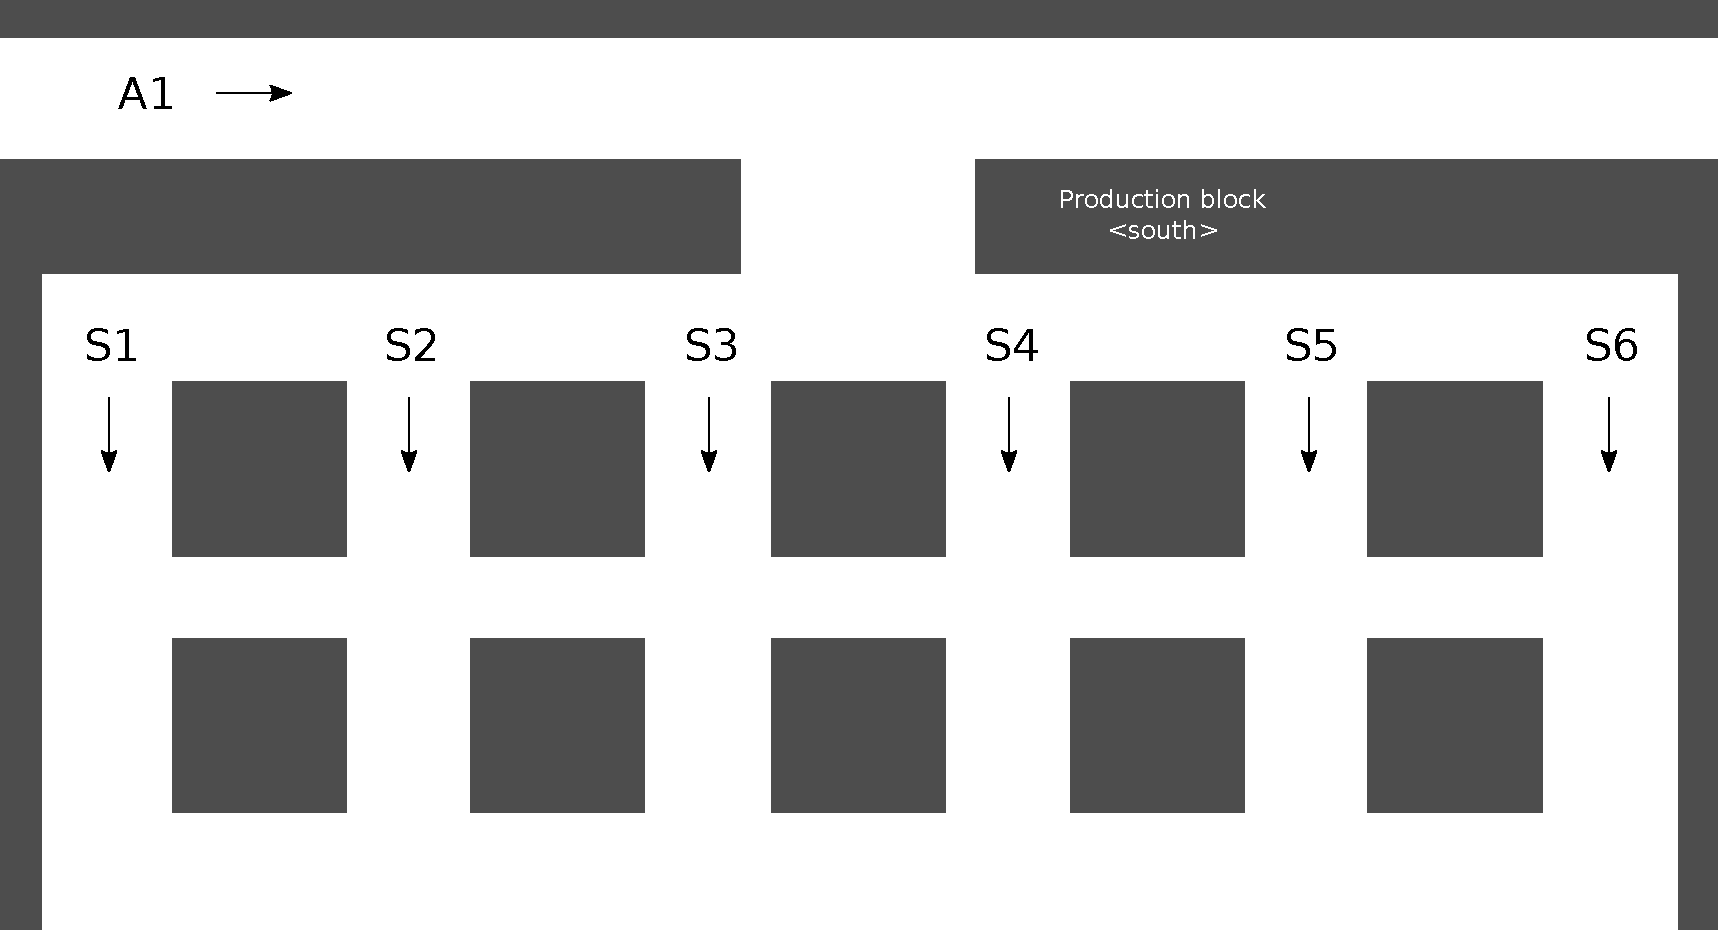
\includegraphics[width=\textwidth]{pictures/room_and_pillar_scheme.pdf}
\centering
\caption{Naming convention in room and pillar production block.}
\label{fig:room_and_pillar_scheme}
\end{figure}

Corridors layout can also invole different levels. Figure \ref{fig:mine_with_levels_scheme} depicts example of such layout. On each floor there are placed room and pillar production blocks. Naming convention for corridors are the same like in room and pillar case. The way down is also a kind of a corridor with a constant, steep angle. Device which is inside of such corridor can be located by the corridor name and the meter counted from the begging on a top level.

\begin{figure}[ht]
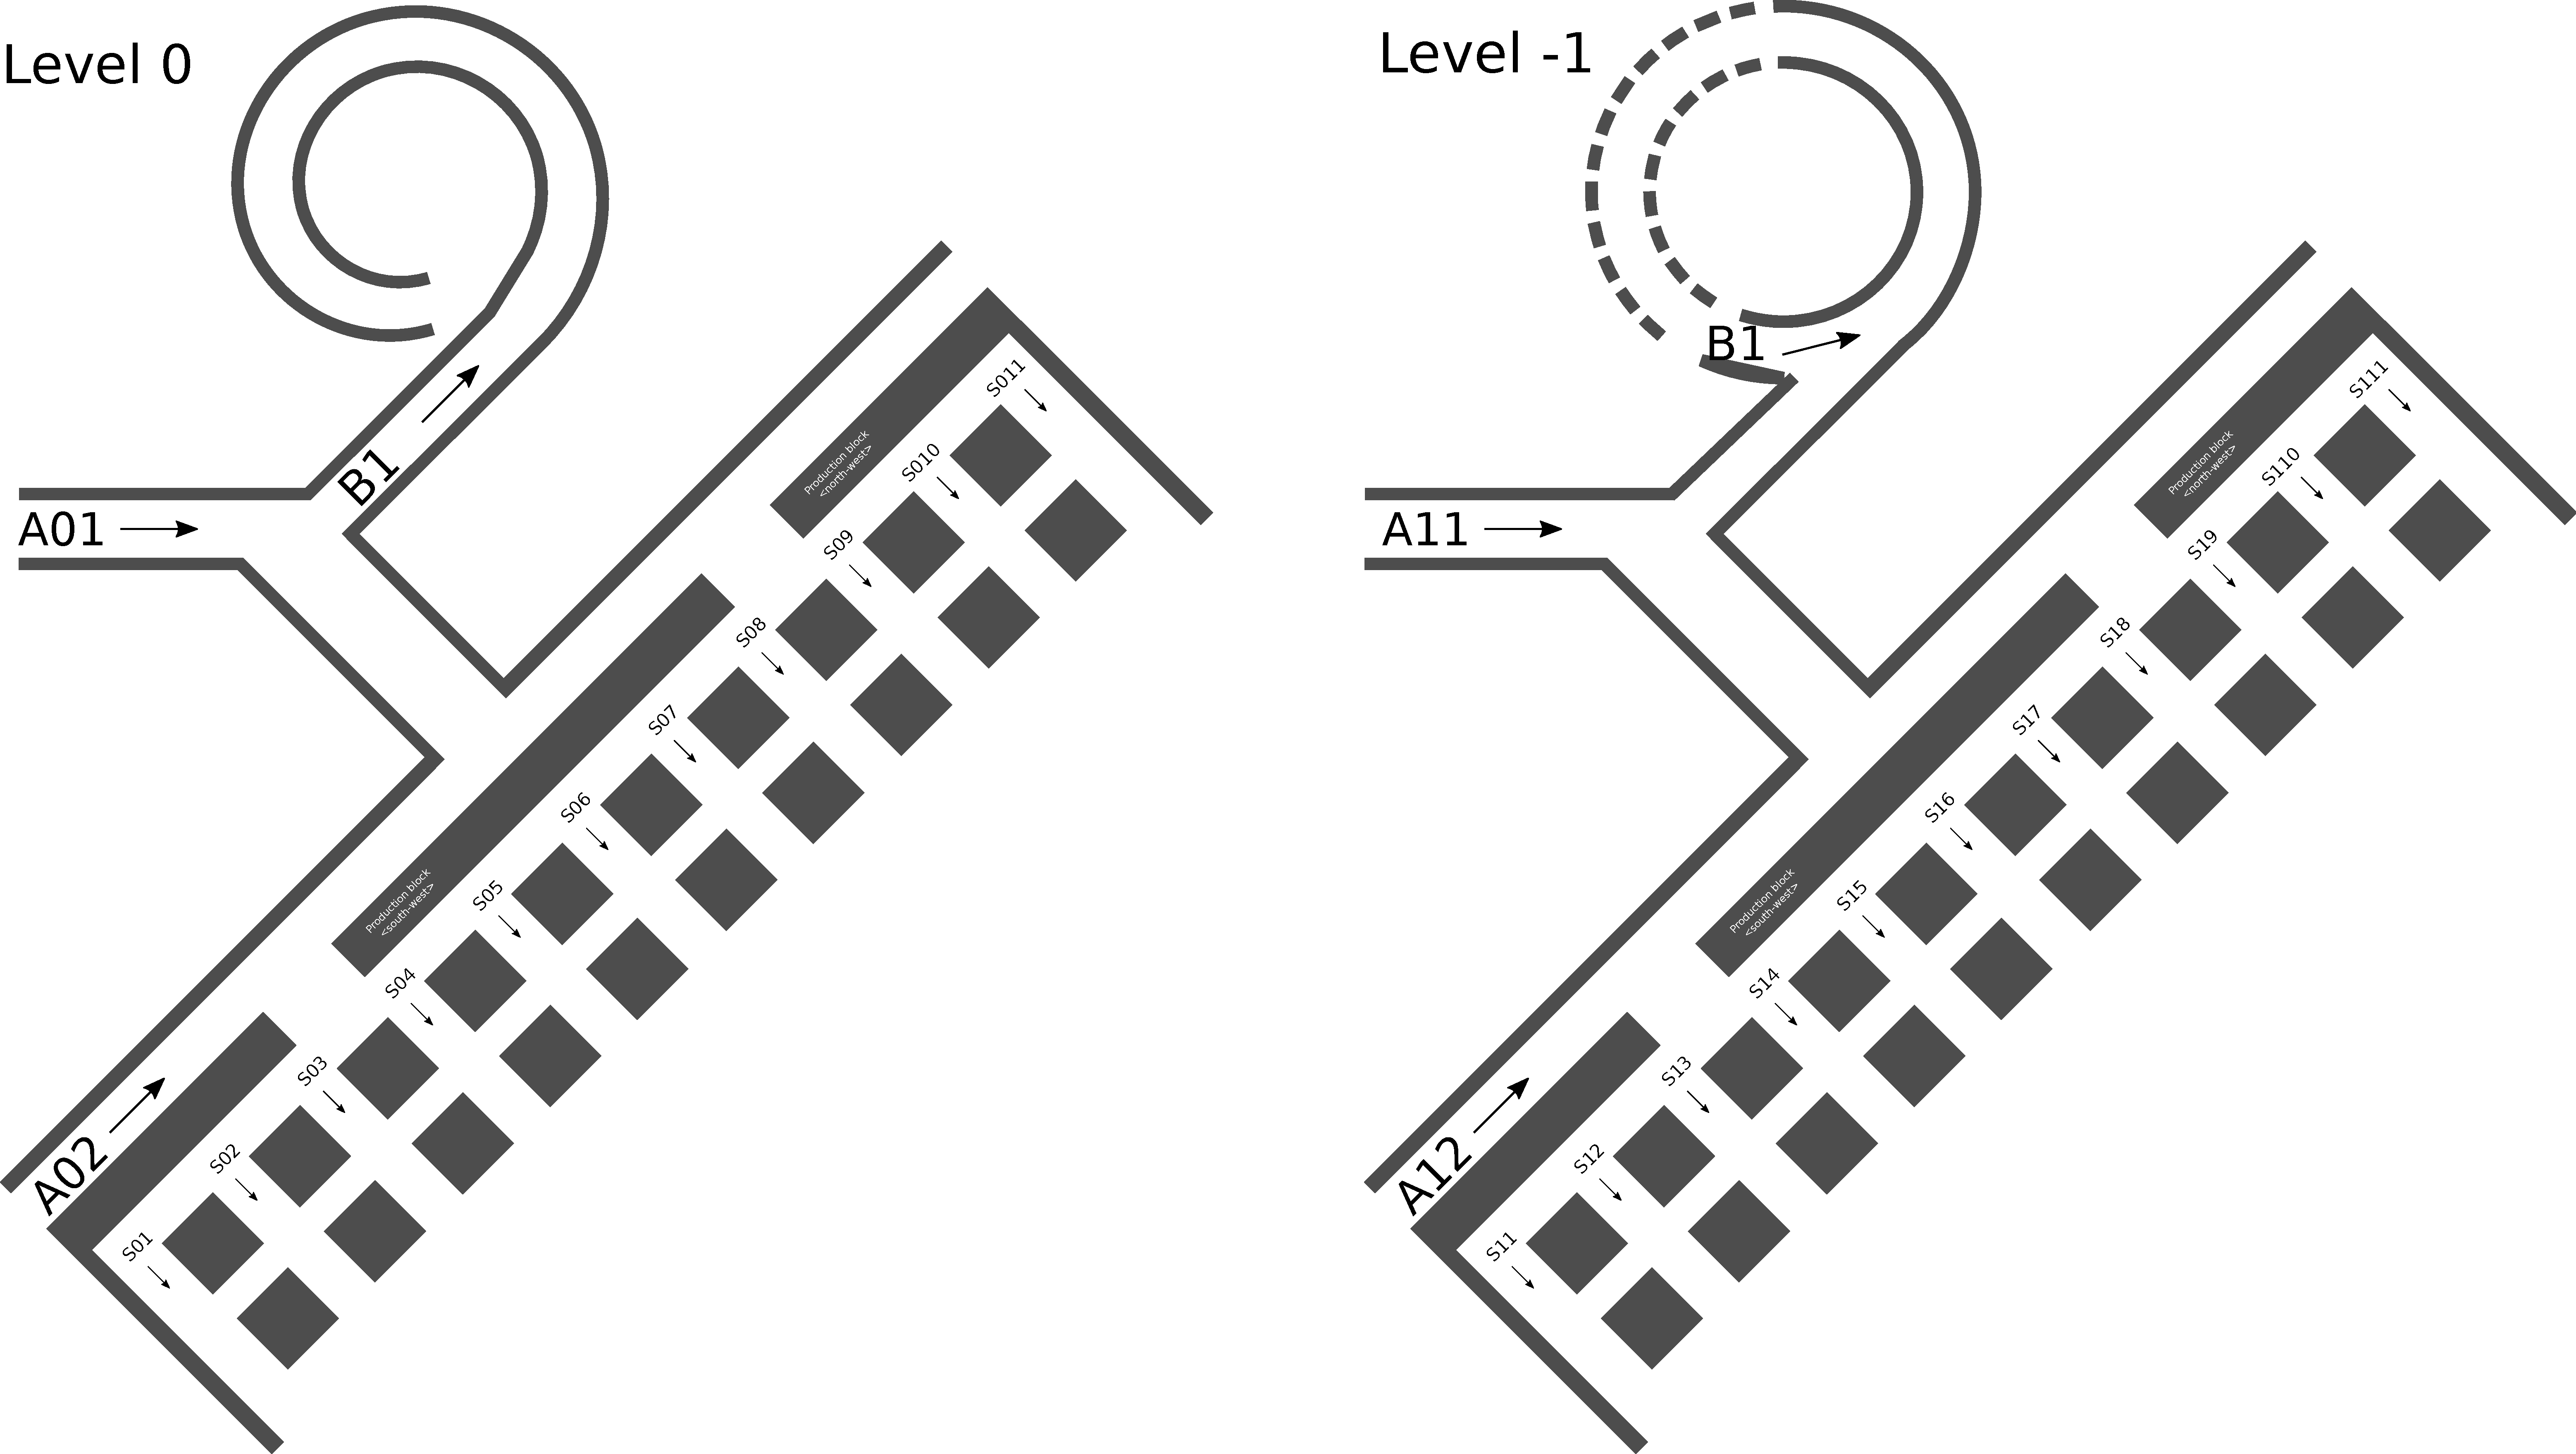
\includegraphics[width=\textwidth]{pictures/mine_with_levels_scheme.pdf}
\centering
\caption{Multi-level corridors layout and example naming convention.}
\label{fig:mine_with_levels_scheme}
\end{figure}


\section{Hardware and environmental constratins} % (fold)
\label{sub:hardware_and_environmental_constratins}



State of the art in underground navigation solutions. Theoretical topic.

Phisics related to waves propagation in underground corridor
\begin{itemize}
	\item Waves difraction, <tłumienie>
	\item What are known issues related to wireless communication in underground installations
\end{itemize}



*TO be adapted; book-wcin
Requirements stated for communication system for the undeground operations:
\begin{itemize}
	\item must be intrinsically safe and explosion proof
	\item should adhere to the ingress protection (IP) standards;
	\item must be rugged in structure
	\item must be size flexible
	\item must have totality in design including cables, power supply unit, base stations, etc
	\item must be value-added priced;e stations, etc
	\item must be robust, inexpensive, easy to expand,
and enable fast and secure connections
\end{itemize}



***
The wireless communication systems used on surface cannot be applied straightaway in underground mines due to high attenuation of radio waves in underground strata. Undergorund radio waves propagation envioronment differ also because of
\begin{itemize}
	\item presence of inflammable gases,
	\item hazardous environment,
	\item complex corridors topology (mines case),
	\item complex geological structures,
\end{itemize}


% subsection hardware_and_environmental_constratins (end)
\section{Positioning systems}

The position finding problem can be categorised with respect of the nature of those problems as well as related solution approaches.

In order to perform categorisation there is need to introduce terms of node, anchor and user. Node is an element of a network or infrastructure, that can take actively part in solving the problem of a localisation. Example of a node can be wireless device that is suited to be a part of WSN network. More details about WSN networks in section \ref{sub:wsn_based_position_finding_systems}. Anchor is a node which position is already known. Anchor plays a role of a reference point that can be used for obtaining the position of nodes or users. User is a mobile entity that is not a part of a infrastructe but make use of it in order to obtain positioning information for himself.

Position finding problems are problems of:
\begin{itemize}
 	\item nodes localisation, where the main interest is to obtain position of entities that build up infrastructure,
 	\item users localisation, where the main interest is to obtain position of mobile entities basing on the infrastructure,
 	\item nodes and users localisation, where there is need to obtain position of nodes and users at the same time.
 \end{itemize}
Figure \ref{fig:localisation_approaches} introduces also a categorisation with respect of the fact that position of anchors and nodes are static or can change in time. As it is depicted, localisation of users problem crossects with the localisation of nodes problem in cases where nodes are a mobile entities. Localisation of users and nodes at the same time is a problem which is mainly related to the filed of robotics where no information about the evironment are provided at once. There are investigated solutions for that sort of problems, called Simultaneous Localisation and Configuration (SLAC) and Simultaneous Localisation and Mapping (SLAM) \cite{discover_beacons_and_position}.

\begin{figure}[ht]
 % trim={<left> <lower> <right> <upper>}
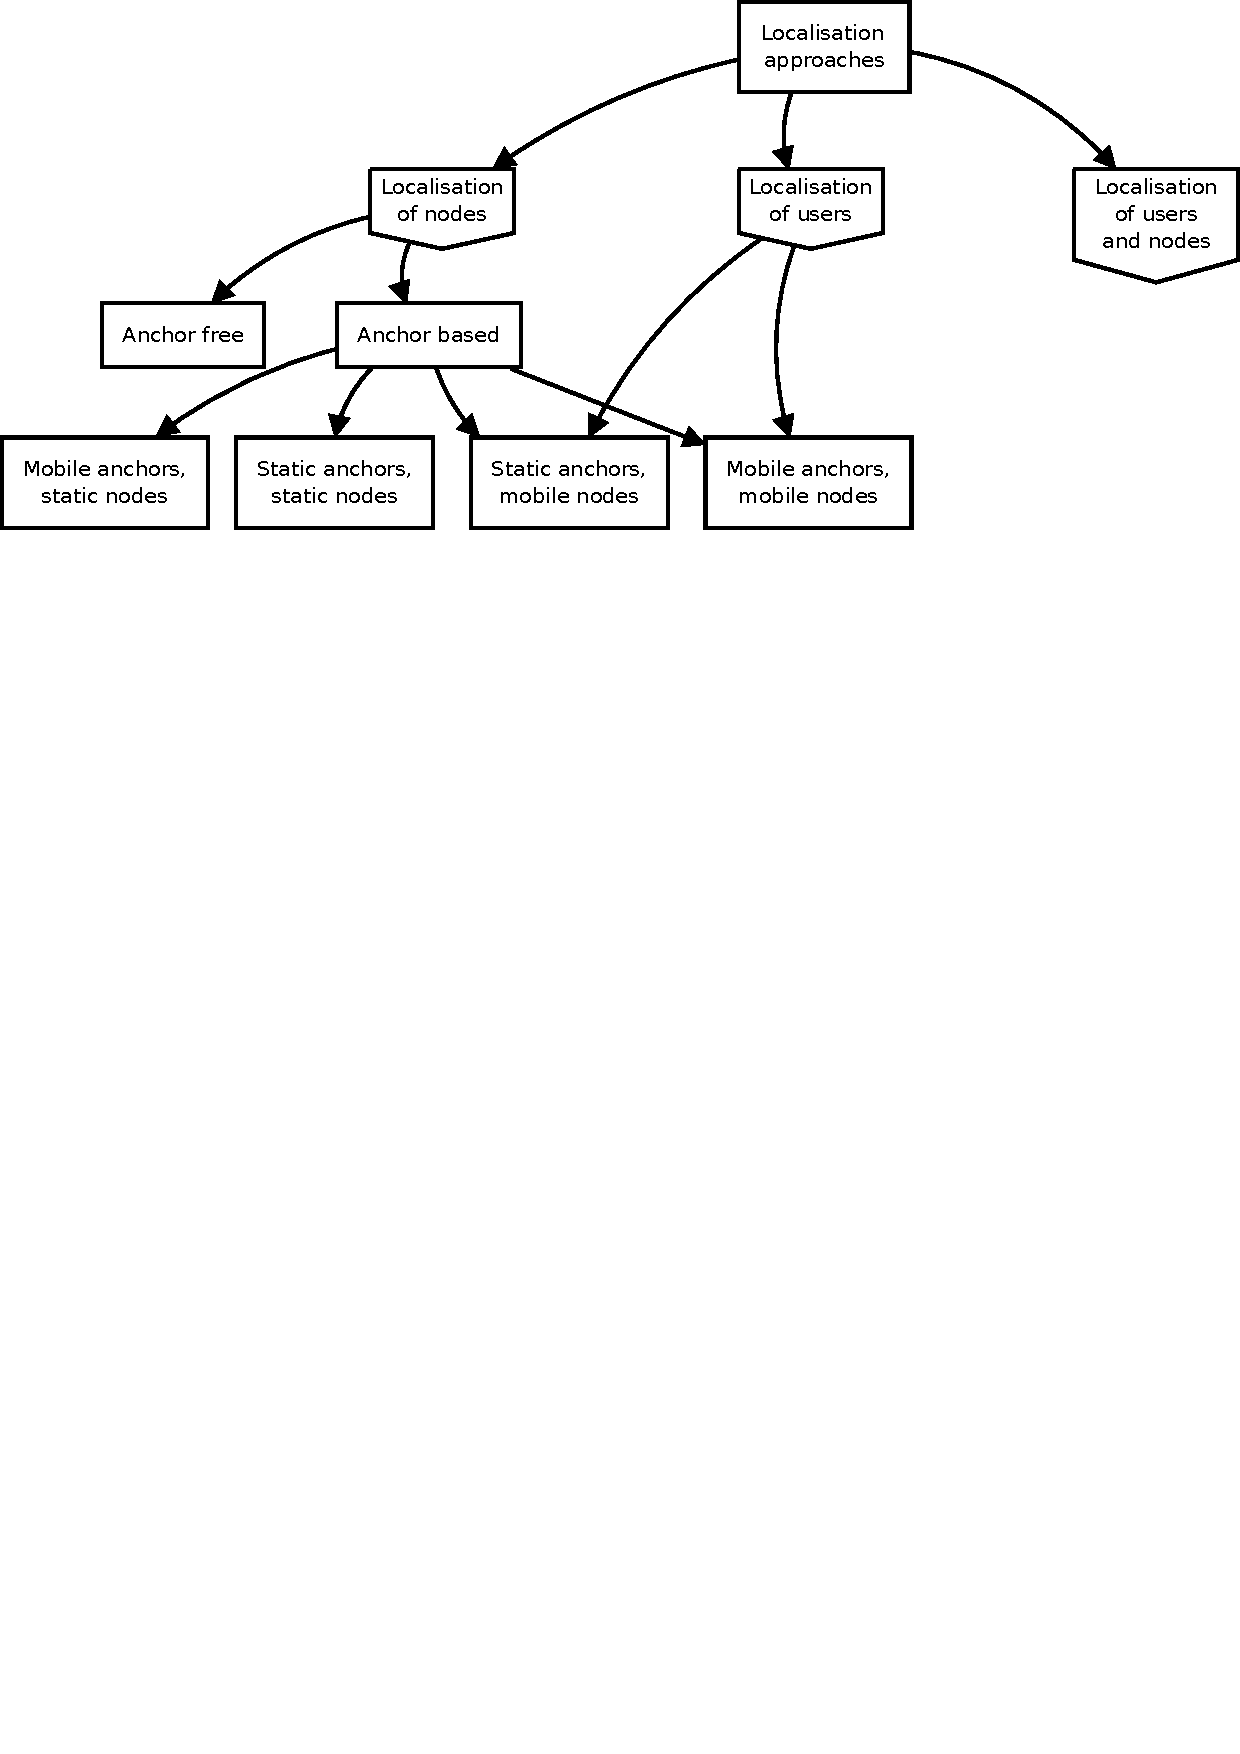
\includegraphics[width=\textwidth, trim={0 20cm 0 0},clip]{pictures/localisation_approaches.pdf}
\centering
\caption{Categorisation of localization problems and related solution approaches\cite{discover_beacons_and_position}.}
\label{fig:localisation_approaches}
\end{figure}

Within this paper there is investigated problem of user localisation only. Solutions for that problem are descibed in details in chapter \ref{chapter:position_finding_solutions}.

Position finding in underground installations is a problem that arrised along with the advance in the available technologies. There is big demand on the market of underground installations for such functionality, There two main applications of position finding solutions:
\begin{itemize}
	\item workers safety,
	\item extension to the task management, monitoring, resource planning and distribution tools.
\end{itemize}


\subsection{Safety aspect} % (fold)
\label{sub:safety_aspect}

Protecting and rescueing people lifes are one of the most important challanges for the underground construction and mining industry since many years. In case of accident there is need to perform appropriate search and rescue actions immediatley as the survival rate decreases rapidly as time passes. As for underground construction and mining industry positioning systems are rather in research stage then in real use, executives doesn't know exact position af miners before accident and how many of them are trapped and how big is the scale of destruction. Currently used techniques for rescueing people after an accident requires to count people that came out to know how many people are trapped and then digg though the falled corridors and perform searching operations that rely on old low frequency technology like GLON. GLON is a polish old low frequency radio solution for finding signal emmited from miners lamp, allowing on detection from a few meters \cite{GLON}. Personal safety equipment consists of oxygen masks enabling to survive 50 minutes, and lamps with GLON transmitter. In case of accident in copper mine "Rudna" in Poland that had a place on 29'th November, 2016  \cite{newspaper_rudna} rescue action started 20 minutes after rock mass movement. Part corridor with chamber for mobile machines and excavation got collapsed. After 1,5 hour it was discovered that there are trapped miners. Rescue team had to dig fallen rocks from both sides of corridor without knowledge where trapped miners are because steel elements from collapsed corridor housing influenced the GLON system measures. Positioning system with online underground monitoring would give immediate information who and were was in time of accident and speed up rescueing operations. Unfortunately there was no such system. Current safety regulations does not take new technology into account. Mines do not know where exactly their miners are, they know only the region.

Modern emergency systems for underground installations provide a set of functions that improves safety and minimise loss in case of accident. Besides the means of emergency situation prevention like preditions of mass movements or presence of gasses, lots of them provide functions that help coordinate miners if they are in the isolated areas to meet each other, guide them to the emergency equipment, exit points or safe areas and ensure that nobody was left in danger place \cite{Thesis_CM}. All of those functions requires good position finding solution in order to provide fast and realiable information even if connectivity is broken.

Positioning system can be used also by people working underground directly from their personal digital equipment\cite{Thesis_CM} as a kind of navigation system which can help to evacuate from underground installation. It could provide information about their current position within mine and there would be given informations about dangerous areas and recommended escape paths in case of emergency.

Positioning systems dedicated to monitoring workers are called LAMPS -- Location and Monitoring for Personal Safety systems.
% subsection safety_aspect (end)

\subsection{Business aspect} % (fold)
\label{sub:business_aspect}

Another use case for positioning system is that stakeholders want to know where the equipment is placed, how many time it needs to do it's operations, if there are some unplanned breakes in machine work. Delays in case of any underground operations are very costly. Resources monitoring can depict bootlenecks in machine operations may provide informations how to balance the workload in order to make operations smoother and more efficient. Data gathered by positioning systems can be also used in time and cost estimations. Mine stakeholders can see in real time what is the current distribution of equipment what enables them to perform real time coordination of ongoing process parts. In day to day operations information where are located operators and machines can increase production efficency because of less time needed to spend on gethering information about machines position from reports. \cite{thesis_tablet_positioning} The positioning systems are mainly used to deliver information to systems that operates above ground. Todays underground operations are partly or fully automated. The process of the operations is monitored and managed remotely from operation centers on surface. Supervior and control of such operations are similiar to that known on above ground process plants which are controlled by SCADA -- Supervisory Control And Data Acquisition software systems \cite{Thesis_CM}.

Underground construction industry use automation technology heavily in nearly all aspects: safety, work automation, work and environment monitoring, internal and external communication, transport, maintainig ventilation, power or fresh water supply and others. Automated solutions are also used for example to control access to mine like entries for cars and mobile mine machines or for safety purpose to quickly cut off rooms where petrol oil are stored in case of accident or fire detection. Those automated systems can be configured and controlled from places they are mounted under ground or from central systems located above ground where central monitoring and work control take a place. Such centers collect informations distributed by systems and provide information about envioronmental parameters or work performance. Devices and mobile machines that work underground are also connected to that system through means of onboard microcontrollers or computers and wireless network. Thanks to it it is possible to provide to central system work performance information or device health status that can be usefull for service during periodical device checks or repairs. Positioning systems implementations may work togehter with these devices which allows underground operation executives to have a up to date map of current works and processes being in progress. Positioning information can be used also by mobile devices by themselves. Example of devices that make use positioning data are modern mobile machine gateways devices \cite{Thesis_CM} which are kind of black-box devices for big mining machines like loaders. Those devices can use positioning information as a trigger for reports of work efficiency expressed in load - unload cycles (IREDES Performance Profile report).
% subsection business_aspect (end)


Nowadays there are available positioning systems for underground installations that can provide aproximate localization of people or equipment.



\section{Usage of mobile devices in underground installations}
Define 'mobile device'

Answer questions:
\begin{itemize}
	\item If mobile device (smartphone class) can be used in undergorund installations?
	\item How usage of mobile device in underground installations may differ from usage in normal conditions (outside underground installation)?
\end{itemize}

\end{document}
